\section{Lecture 1}

\subsection{Motivation}

To study the geometry of a complex variety $X/\CC$ it is often useful to put it
into a family and to study the other fibres
\[
	f \colon \mathfrak{X} \to \Aff^{1}_{\CC}
\]
such that $X \cong f^{-1}(a)$ for some $a$.

Typical situation: $X$ is smooth and proper over $\CC$. Then one might take
$\mathfrak{X}$ regular, $f$ proper and flat, and such that all singular fibres
of $f$ are strict normal crossings divisors.
(Strict normal crossings divisors means that locally they look like unions of
coordinate hyperplanes.)
\begin{center}
	\begin{tikzpicture}[every node/.style={font=\small}]
		\draw (-2,2) node[left] {$\mathfrak{X}$} -- (-2,0) -- (2,0);
		\draw (-2,-.7) node[left] {$\Aff^{1}_{\CC}$} -- (2,-.7);
		\draw[->] (-2.25,1.6) -- node[left] {$f$} (-2.25,-.2);
		\draw (-.5,2) node[above] {$X = \mathfrak{X}_{a}$} -- (-.5,.1);
		\draw (1.5,2) node[above] {$\mathfrak{X}_{0}$} -- (1.5,.1);
		\draw (1.3,1.6) to [controls=+(0:.8) and +(0:.8)] (1.3,0.9);
		\draw[fill] (-.5,-.7) circle (.01) node[below] {$\tau = a\vphantom{0}$};
		\draw[fill] (1.5,-.7) circle (.01) node[below] {$\tau = 0$};
	\end{tikzpicture}
\end{center}
\begin{idea}
	The geometric complexity of $X$ is reflected in the geometric
	complexity of $\mathfrak{X}_{0}$.

	If we want to study the degeneration of the family at a particular
	fibre $\mathfrak{X}_{0}$, we can zoom in around $\mathfrak{X}_{0}$ by
	base changing to $\widehat{\mathcal{O}_{\Aff^{1}_{\CC,0}}} = \CC[[T]]$.

	So we want to study schemes over discrete valuation rings.
\end{idea}

\begin{notation}
	\begin{itemize}
		\item[$R$] discrete valuation ring
		\item[$t$] local uniformizer (i.e., generator of the maximal ideal)
		\item[$k$] residue field (we assume $k = \bar{k}$)
		\item[$K$] fraction field
	\end{itemize}
\end{notation}

\begin{example}
	There are two cases.
	\begin{itemize}
		\item The \emph{equal} characteristic case: $R = k[[t]]$, $K = k((t))$.
		\item The \emph{mixed} characteristic case: $R = \widehat{\ZZ_{p}^{\nr}} = W(\FF_{p})$, $K = \widehat{\QQ_{p}^{\nr}}$, $t = p$. (In general $R$ is a finite extension of $W(k)$.)
	\end{itemize}
\end{example}
The geometric picture corresponding to this is
\begin{itemize}
	\item[$\Spec(R)$] ``small disk around $0 \in \CC$''
	\item[$t$] ``coordinate on this disk''
	\item[$\Spec(K)$] ``small punctured disk around $0 \in \CC$''
\end{itemize}

Let $X$ be a smooth proper geometrically connected variety over $K$.
Geometrically we can think of a family of connected smooth proper varieties
over a punctured disk.
\begin{definition}
	A \emph{model for $X$ over $R$} is a proper and flat $R$-scheme $\mathfrak{X}$ together with an isomorphism $\mathfrak{X}_{K} \to X$.

	A morphism of models $\mathfrak{Y} \to \mathfrak{X}$ is an $R$-morphism such that
	\[
		\begin{tikzcd}[column sep=small]
			\mathfrak{Y}_{K} \ar{rr} \drar[near start,sloped]{\sim}
			&& \mathfrak{X}_{K} \dlar[near start,swap,sloped]{\sim} \\
			& X
		\end{tikzcd}
	\]
	commutes.
\end{definition}
Note: There exists at most one morphism from $\mathfrak{Y}$ to $\mathfrak{X}$.
If such a morphism exists, we say that $\mathfrak{Y}$ dominates $\mathfrak{X}$.
We say that $\mathfrak{X}$ is an \emph{snc-model} if $\mathfrak{X}$ is regular
and $\mathfrak{X}_{k}$ is a strict normal crossings divisor, i.e., for every $x
\in \mathfrak{X}$, there exists a regular system of local parameters
\emph{(i.e., a basis of the Zariski tangent space)} $(Z_{1}, \ldots Z_{d})$ and
a unit $u$ in $\mathcal{\mathfrak{X},x}$ such that $t = uZ_{1}^{N_{1}} \cdots
Z_{d}^{N_{d}}$ for some $N_{i} \ge 0$. We say that $\mathfrak{X}$ is an
\emph{nc-model} if $\mathfrak{X}$ is regular and $\mathfrak{X}_{k}$ is a normal
crossings divisor, i.e., an snc-divisor for the étale topology. This ``allows
for self-intersections''.
\begin{center}
	\begin{tikzpicture}[every node/.style={font=\small}]
		\draw (0,0) to [controls=+(110:3) and +(250:3)] (0,1);
		\path (0,.5) node[right] {nc, but not snc};

		\draw[->] (-.5,-1.2) -- node[right] {étale} (-.5,-.4);

		\begin{scope}[yshift=-2.5cm]
			\draw (0,0) to [controls=+(180:1) and +(180:1)] (0,1);
			\draw (0,.1) to [controls=+(200:2) and +(160:2)] (0,.9);
		\end{scope}
	\end{tikzpicture}
\end{center}

The variety $X$ always has an $R$-model, by Nagata's embedding theorem.
\[
	\begin{tikzcd}
		X \dar{\text{proper}} \rar[hook]{\exists} & \mathfrak{X} \dar \\
		\Spec(K) \rar[hook] & \Spec(R)
	\end{tikzcd}
\]
The existence of nc-/snc-models is much more subtle and relies on
\emph{resolution of singularities}. This is expected to be true in general by
most experts; but currently we know:
\begin{itemize}
	\item $\chr(k) = 0$: holds for all $X$ (Hironaka, 1964)
	\item $\chr(k) > 0$: holds if $\dim(X) = 1$ (Lipman, 1978)
	\item $\chr(k) > 0$: holds if $\dim(X) = 2$ (Cossart--Pikant, last week?)
\end{itemize}
Until further notice, we will assume $\dim(X) = 1$.

\subsection{Intersection theory}

Intersection theory over discrete valuation rings (Lichtenbaum).

Let $X$ be a curve, $\mathfrak{X}$ a regular model of $X$. A divisor $E =
\sum_{i=1}^{n} a_{i}E_{i}$ is \emph{vertical} if it is supported on
$\mathfrak{X}_{k}$. (In particular, then $E$ is proper over $k$.)

\begin{figure}
	\caption{The distinction between horizontal and vertical divisors}
	\label{horvertdivs}
	\begin{center}
		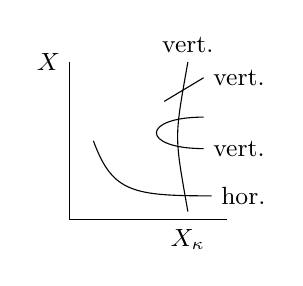
\begin{tikzpicture}[every node/.style={font=\small}]
			\draw (0,2) node[left] {$\mathfrak{X}$} -- (0,0) -- (2,0);
			\draw (1.5,2) node[above] {vert.} to[controls=+(260:1) and +(100:1)] (1.5,.1);
			\draw (1.2,1.5) -- (1.7,1.8) node[right] {vert.};
			\draw (1.7,1.3) to [controls=+(180:.8) and +(180:.8)] (1.7,0.9) node[right] {vert.};
			\draw (.3,1) to[controls=+(290:.7) and +(180:1)] (1.8,.3) node[right] {hor.};
			\path (1.5,0) node[below] {$\mathfrak{X}_{\kappa}$};
		\end{tikzpicture}
	\end{center}
\end{figure}

Let $E = \sum_{i=1}^{n} a_{i}E_{i}$ be a vertical divisor, and $D$ any divisor.
The intersection product is defined as:
\[
	(D \cdot E) = \sum_{i=1}^{n} a_{i} \deg \mathcal{O}(D)|_{\tilde{E_{i}}},
\]
where $\tilde{E_{i}} \to E_{i}$ is the normalisation.

The intersection product has the following properties:
\begin{itemize}
	\item It coincides with the geometric intuition if $D$ and $E$ have no common components.
	\item It is bilinear.
	\item It is symmetric if $D$ is vertical.
	\item It is invariant under linear equivalence on $D$.
	\item It is \emph{not(!)} invariant under linear equivalence on $E$.
		For example $\mathfrak{X}_{k} \sim 0$, but $(D \cdot
		\mathfrak{X}_{k}) \ne 0$ if $D$ consists of one horizontal
		component. See for example \cref{horvertdivs}.
	\item Behaviour under morphisms: If $h \colon \mathfrak{Y} \to
		\mathfrak{X}$ is a morphism of models, then
		\begin{center}
			\begin{tabular}{ll}
				$(D \cdot h^{*}E) = (h_{*}D \cdot E)$ &
				$(h^{*}D \cdot E) = (D \cdot h_{*}E)$ \\
				$D$ on $\mathfrak{Y}$ & $D$ on $\mathfrak{X}$ \\
				$E$ vertical on $\mathfrak{X}$ & $E$ vertical on $\mathfrak{Y}$
			\end{tabular}
		\end{center}
		which also imply $(h^{*}D \cdot h^{*}E) = (D \cdot E)$, when
		$D$ is a divisor on $\mathfrak{X}$, and $E$ a vertical divisor
		on $\mathfrak{X}$.
\end{itemize}

If $D$ is a divisor on a regular model $\mathcal{X}$ of $X$, then 
\[
(D \cdot \mathcal{X}_{k}) = \mathrm{deg}(D|_{X}).
\]
\begin{exercise}
	Prove this.
\end{exercise}
